\section{}
A simple wooden beam is under a uniform load of intensity $p$, as illustrated in Fig. \ref{fig:Q6ProblemDiagram}.
\begin{figure}[h]
    \centering
    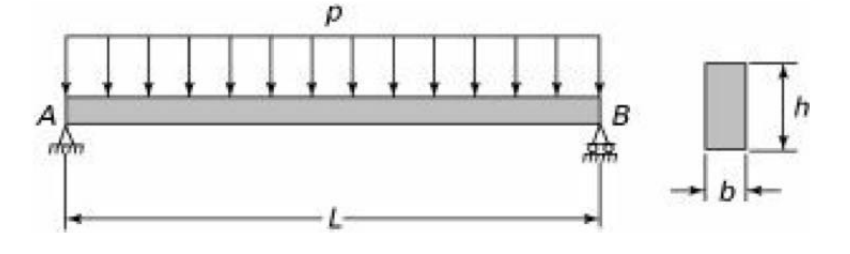
\includegraphics[width=0.35\linewidth]{Questions/Figures/Q6ProblemDiagram.png}
    \caption{Problem diagram for Question 6.}
    \label{fig:Q6ProblemDiagram}
\end{figure}
\begin{enumerate}[label=(\alph*)]
    \item Find the ratio of the maximum shearing stress to the largest bending stress in terms of the
    depth $h$ and length $L$ of the beam.
    \item Using $\sigma_{all} = 9$ MPa, $\tau_{all} = 1.4$ MPa, $b = 50$ mm, and $h = 160$ mm, calculate the maximum
    permissible length $L$ and the largest permissible distributed load of intensity $p$.
\end{enumerate}

Like in Question 5, the shear force and bending moment are given by
\begin{align*}
    V &= \frac{pL}{2} \langle x - 0 \rangle^{0} - p \langle x - 0 \rangle^{1} \\
    M & = \frac{pL}{2} \langle x - 0 \rangle^{1} - \frac{p}{2} \langle x - 0 \rangle^{2} \\
\end{align*}

By symmetry, the maximum bending moment occurs at the center of the beam. From inspection, the max shear force is at the supports. Then,
\begin{align*}
    V_{\max} &= \frac{pL}{2} \\
    M_{\max} &= \frac{pL^2}{8}
\end{align*}

Then,
\begin{align*}
    \sigma_{\max} &= \frac{M_{\max} y}{I_z} = \frac{pL^2 h/2}{8 bh^3/12} \\
    &= \frac{3pL^2}{4bh^2} \\
    \tau_{\max} &= \frac{3V_{\max}}{2A} = \frac{3pL}{4bh} \\
    \frac{\tau_{\max}}{\sigma_{\max}} &= \boxed{\frac{h}{L}}    
\end{align*}
\begin{lstlisting}[language=Matlab]
syms p L b h
sigma_max = 3*p*L^2/(4*b*h^2);
tau_max = 3*p*L/(4*b*h);
ratio = tau_max/sigma_max;
\end{lstlisting}
